\documentclass{ctexart}
\pagestyle{empty} % 禁用页眉页脚，包括页码
\setlength{\parindent}{2em}
\usepackage[
  paperwidth=17cm,
  paperheight=25cm,
  margin=6pt
]{geometry}
\usepackage{titlesec}

% 调整 \section 标题字号与间距
\titleformat{\section}
  {\normalfont\bfseries\large} % 样式：\Large 可改为 \huge, \small 等
  {\thesection}{0em}{}         % 编号和间距设置
  \titlespacing{\section}{0pt}{10pt}{0pt}

\usepackage{multicol}  
\usepackage{amsmath} 
\usepackage{amssymb} 
\usepackage{tikz}
\usetikzlibrary{calc}


\newcommand{\TT}{\mathrm{T}}
\begin{document}

\section*{平面二连杆动力学推导}

\begin{center}
    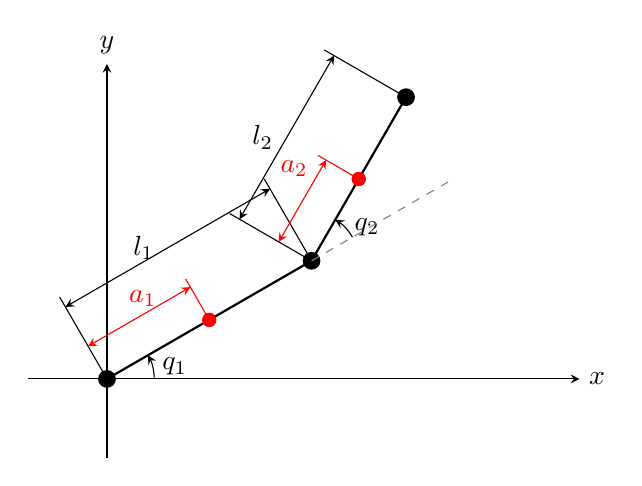
\begin{tikzpicture}[scale=2, >=stealth]
        % 坐标系
        \draw[->] (-0.5,0) -- (3,0) node[right] {$x$};
        \draw[->] (0,-0.5) -- (0,2) node[above] {$y$};

        % 参数
        \def\lone{1.5}    % l1
        \def\ltwo{1.2}    % l2
        \def\aone{0.75}   % a1
        \def\atwo{0.6}    % a2
        \def\thone{30}    % θ1
        \def\thtwo{30}    % θ2
        \def\ext{0.6}    % 引出线长度

        % 关键点
        \coordinate (O) at (0,0);
        \coordinate (J1) at ({\lone*cos(\thone)}, {\lone*sin(\thone)});
        \coordinate (J2) at ({\lone*cos(\thone) + \ltwo*cos(\thone+\thtwo)},
        {\lone*sin(\thone) + \ltwo*sin(\thone+\thtwo)});

        \coordinate (C1) at ({\aone*cos(\thone)}, {\aone*sin(\thone)});
        \coordinate (C2) at ({\lone*cos(\thone) + \atwo*cos(\thone+\thtwo)},
        {\lone*sin(\thone) + \atwo*sin(\thone+\thtwo)});

        % 绘制连杆
        \draw[thick] (O) -- (J1);
        \draw[thick] (J1) -- (J2);

        % 绘制关节
        \filldraw[black] (O) circle (1.5pt);
        \filldraw[black] (J1) circle (1.5pt);
        \filldraw[black] (J2) circle (1.5pt);

        % 绘制质心
        \filldraw[red] (C1) circle (1.2pt);
        \filldraw[red] (C2) circle (1.2pt);

        % 标注 l1 与 a1
        \draw[]
        (O) -- ++({-\ext*sin(\thone)}, {\ext*cos(\thone)})
        coordinate (Oline);
        \draw[]
        (J1) -- ++({-\ext*sin(\thone)}, {\ext*cos(\thone)})
        coordinate (J1line);
        \draw[red]
        (C1) -- ++({-\ext/2*sin(\thone)}, {\ext/2*cos(\thone)})
        coordinate (C1line);
        \draw[<->] ($(O)!0.88!(Oline)$) -- ($(J1)!0.88!(J1line)$)
        node[midway, left, xshift=-0.05cm] {$l_1$};
        \draw[<->, red] ($(O)!0.4!(Oline)$) -- ($(C1)!0.8!(C1line)$)
        node[pos=0.8, left, xshift=-0.05cm] {$a_1$};

        % 标注 l2 与 a2
        \draw[]
        (J1) -- ++({-\ext*sin(\thone+\thtwo)}, {\ext*cos(\thone+\thtwo)})
        coordinate (J1line);
        \draw[]
        (J2) -- ++({-\ext*sin(\thone+\thtwo)}, {\ext*cos(\thone+\thtwo)})
        coordinate (J2line);
        \draw[red]
        (C2) -- ++({-\ext/2*sin(\thone+\thtwo)}, {\ext/2*cos(\thone+\thtwo)})
        coordinate (C2line);
        \draw[<->] ($(J1)!0.88!(J1line)$) -- ($(J2)!0.88!(J2line)$)
        node[midway, left, xshift=-0.05cm] {$l_2$};
        \draw[<->, red] ($(J1)!0.4!(J1line)$) -- ($(C2)!0.8!(C2line)$)
        node[pos=0.9, left, xshift=-0.05cm] {$a_2$};

        % 绘制角度标记
        \draw[->] (0.3,0) arc (0:\thone:0.3) node[midway, right] {$q_1$};
        \draw[->] ({(\aone + 0.15)*2*cos(\thone)}, {(\aone + 0.15)*2*sin(\thone)}) arc (\thone:\thone+\thtwo:0.3) node[midway, right] {$q_2$};
        \draw[gray, dashed] (J1) -- ++({cos(\thone)}, {sin(\thone)});

    \end{tikzpicture}
\end{center}

模型定义见上图，其中 $q_1, q_2$ 为关节角，$l_1, l_2$ 为连杆长度，$a_1, a_2$ 为各连杆质心到其起点的距离。设 $m_1, m_2$ 为连杆质量，$I_1, I_2$ 为绕质心的转动惯量，$g$ 为重力加速度。

两连杆质心速度的雅可比矩阵分别为
\[
    J_1 =
    \begin{bmatrix}
        - a_1 \sin q_1    & 0 \\
        \;\; a_1 \cos q_1 & 0
    \end{bmatrix},
\]

\[
    J_2 =
    \begin{bmatrix}
        - l_1 \sin q_1 - a_2 \sin(q_1 + q_2)    & - a_2 \sin(q_1 + q_2)    \\
        \;\; l_1 \cos q_1 + a_2 \cos(q_1 + q_2) & \;\; a_2 \cos(q_1 + q_2)
    \end{bmatrix}.
\]

系统动能可由雅可比矩阵表示为：
\begin{align*}
    T & =
    \frac{1}{2} m_1 \dot{\boldsymbol q}^\TT J_1^\TT J_1 \dot{\boldsymbol q}
    + \frac{1}{2} m_2 \dot{\boldsymbol q}^\TT J_2^\TT J_2 \dot{\boldsymbol q}
    + \frac{1}{2} I_1 \dot{q}_1^2
    + \frac{1}{2} I_2 (\dot{q}_1 + \dot{q}_2)^2                                            \\
      & = \frac{1}{2}\dot{\boldsymbol q}^\TT \left(m_1 J_1^\TT J_1 + m_2 J_2^\TT J_2 + I_1
    \begin{bmatrix}
            1 & 0 \\
            0 & 0
        \end{bmatrix}
    + I_2
    \begin{bmatrix}
            1 & 1 \\
            1 & 1
        \end{bmatrix}\right) \dot{\boldsymbol q}                                               \\
      & = \frac{1}{2} \dot{\boldsymbol q}^\TT M(\boldsymbol q)\, \dot{\boldsymbol q}
\end{align*}

势能为：
\[
    V = m_1 g y_1 + m_2 g y_2.
\]

由动能表达式可得质量矩阵 $M(\boldsymbol q)$ 展开为
\[
    M(\boldsymbol q) =
    \begin{bmatrix}
        M_{11} & M_{12} \\
        M_{21} & M_{22}
    \end{bmatrix}, \quad
    \left\{
    \begin{aligned}
        M_{11} & = m_1 a_1^2 + I_1
        + m_2 \bigl(l_1^2 + a_2^2 + 2 l_1 a_2 \cos q_2\bigr) + I_2,        \\
        M_{12} & =M_{21} = m_2 \bigl(a_2^2 + l_1 a_2 \cos q_2\bigr) + I_2, \\
        M_{22} & = m_2 a_2^2 + I_2
    \end{aligned}
    \right.
\]

科氏力与离心力项可写为
\[
    C(\boldsymbol q, \dot{\boldsymbol q}) \dot{\boldsymbol q} =
    \begin{bmatrix}
        c (2\dot{q}_1 \dot{q}_2 + \dot{q}_2^2) \\
        \;\; -c \dot{q}_1^2
    \end{bmatrix},
    \quad
    c = m_2 l_1 a_2 \sin q_2.
\]

重力项为
\[
    G(\boldsymbol q) =
    \begin{bmatrix}
        (m_1 a_1 + m_2 l_1) g \cos q_1 + m_2 a_2 g \cos(q_1 + q_2) \\
        m_2 a_2 g \cos(q_1 + q_2)
    \end{bmatrix}.
\]

二连杆系统的拉格朗日动力学方程最终可写为
\[
    M(\boldsymbol q)\, \ddot{\boldsymbol q}
    + C(\boldsymbol q, \dot{\boldsymbol q})\, \dot{\boldsymbol q}
    + G(\boldsymbol q)
    =
    \boldsymbol \tau,
\]

\end{document}
